\section{Models} \label{sec:theory_theory_models}
The game includes two characters and a car. \todo{Might want to add a subsection for the car. In that case we should remove line 4.}
Both characters use the same model, and the same texture with different colors.
The car is simpler than the characters as it does hot have any animations.
Because of that this section will only focus on the player model.

The model can be divided into two parts.
The mesh part and the animation part.
What the two parts have in common is that they are both created in Blender, exported to a COLLADA file and loaded into the game using AssimpNet.
Both of these parts are described in this section.


\subsection{Model Mesh} \label{sec:theory_theory_models_mesh}
The model mesh contains the vertices, normals, texture coordinates and indices of the model.
The vertices are the points that make up the model and the normals are automatically assigned by Blender.
The texture coordinates are the coordinates of the texture that is mapped onto the model.
The texture however is a two dimensional image and the model is three dimensional so the mapping is not trivial.
The model mesh has seams that define how a mesh is unwrapped.
These are selected edges that are marked as seams in Blender.
Cutting along these seams will result in a set of faces that can be laid out flat.
This is called the UV map.
This is how the texture is mapped onto the model.
A UV map is shown in \autoref{fig:uv_map}.
For example, the helmet is cut into two parts (the front and the back) and laid out flat in the top right corner of the texture.
This texture describes the color of each pixel of the model.
The whole model can be seen in \autoref{fig:player_model}.

\begin{figure}[h]
    \centering
    \begin{subfigure}{0.45\textwidth}
        \centering
        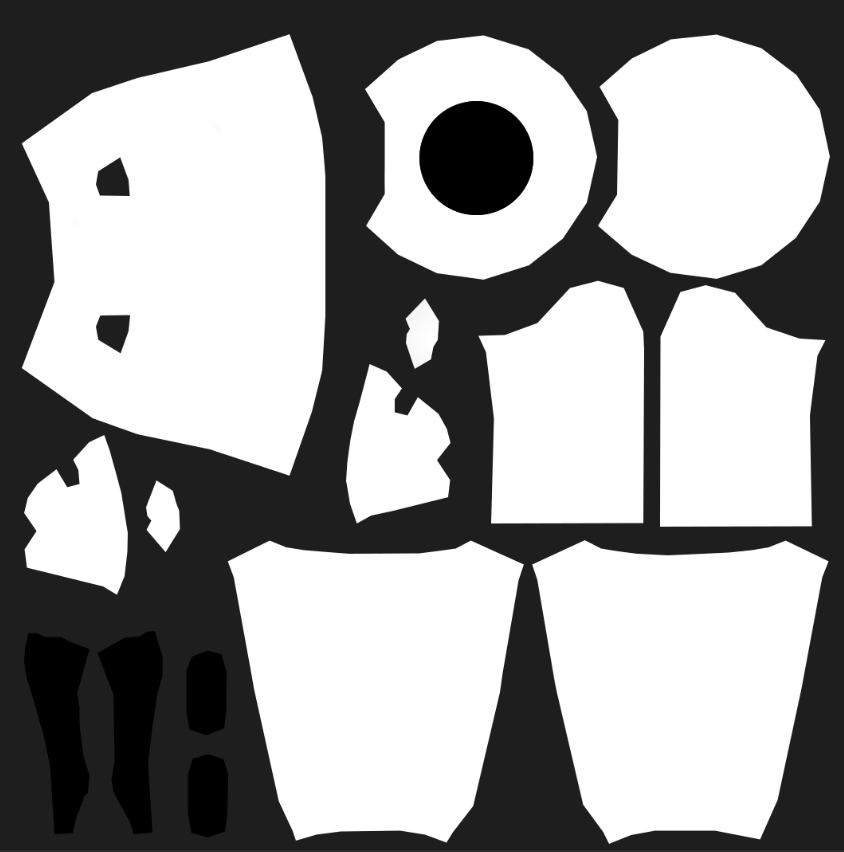
\includegraphics[width=0.8\textwidth]{chapters/theoretical_foundations/sections/models/resources/Texture.png}
        \caption{UV map}
        \label{fig:uv_map}
    \end{subfigure}
    \hfill
    \begin{subfigure}{0.45\textwidth}
        \centering
        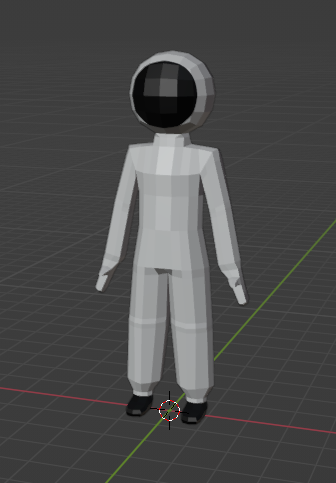
\includegraphics[width=0.8\textwidth]{chapters/theoretical_foundations/sections/models/resources/Model.png}
        \caption{Player model}
        \label{fig:player_model}
    \end{subfigure}

    \caption{Player model and the texture.}
\end{figure}

\subsection{Model Animation} \label{sec:theory_theory_models_animation}
The model animations make use of the model armature (skeleton) which can be seen in \autoref{fig:armature}.
The armature is a set of bones that have different relations to each other and to the mesh.
The bones create a node structure with the root being the torso bone.
Most other bones are children of the torso bone or children of children of the torso bone.
This relation allows the bones to inherit transformations from their parents.
For example, if a leg bone moves the foot bone will follow. 

It is worth noting that bone structure does not have to resemble the human bone structure.
For example in \autoref{fig:armature_foot} we can see a set of bones that are outside of the body.
These bones are not used to deform the mesh but to interact with other bones.
Among other things, these guarantee that the knee does not bend in the wrong direction.


\begin{figure}[H]
    \centering
    \begin{subfigure}{0.45\textwidth}
        \centering
        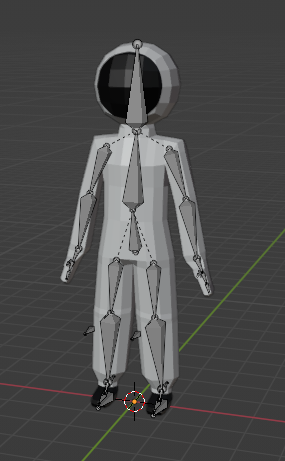
\includegraphics[width=0.8\textwidth]{chapters/theoretical_foundations/sections/models/resources/Armature.png}
        \caption{Armature.}
        \label{fig:armature}
    \end{subfigure}
    \hfill
    \begin{subfigure}{0.45\textwidth}
        \centering
        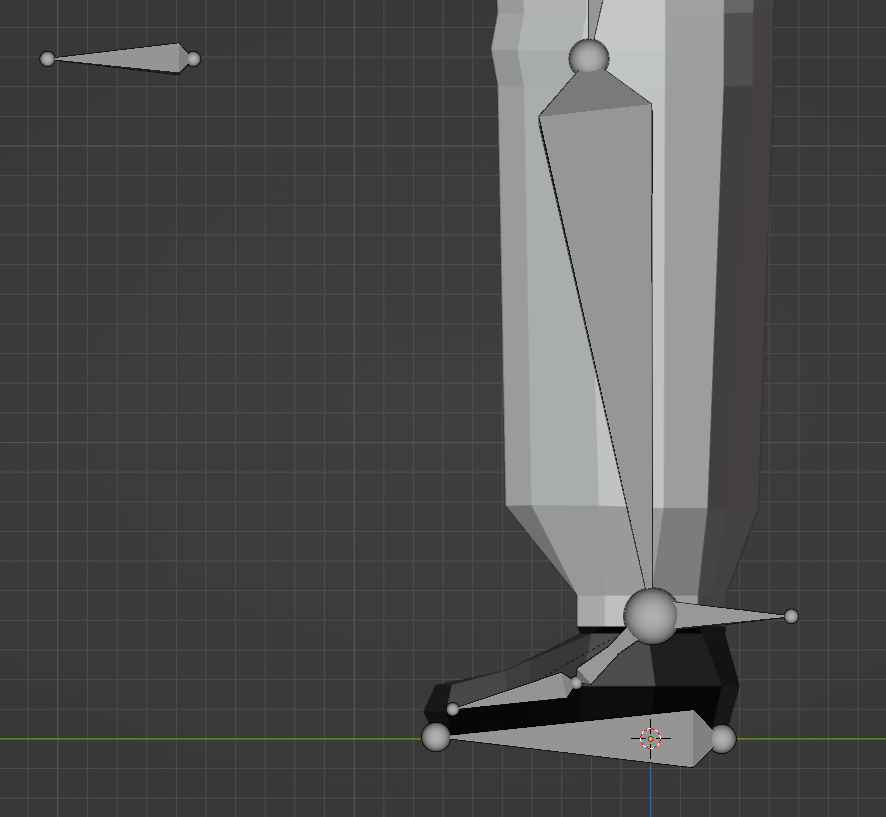
\includegraphics[width=0.8\textwidth]{chapters/theoretical_foundations/sections/models/resources/ArmatureFoot.png}
        \caption{Abnormal bones.}
        \label{fig:armature_foot}
    \end{subfigure}

    \caption{Armature.}
\end{figure}

The bones need to be connected to the mesh.
Each vertex is assigned a set of bones that influence it with different weights.
When bones move the vertices move with them according to how much they move and how much a certain bone influences a certain vertex.
Assigning weights to vertices in Blender is shown in \autoref{fig:vertex_weights}.
As can be seen in the figure, it is done by selecting a bone and then painting the vertices with a certain weight.

\begin{figure}[H]
    \centering
    \begin{subfigure}{0.45\textwidth}
        \centering
        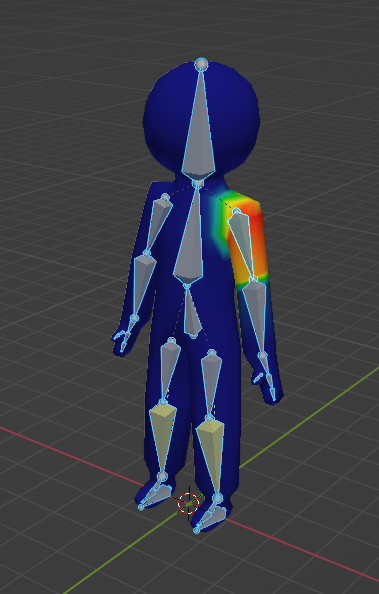
\includegraphics[width=0.8\textwidth]{chapters/theoretical_foundations/sections/models/resources/WeightPaint.png}
        \caption{Vertex weights.}
        \label{fig:vertex_weights}
    \end{subfigure}
    \hfill
    \begin{subfigure}{0.45\textwidth}
        \centering
        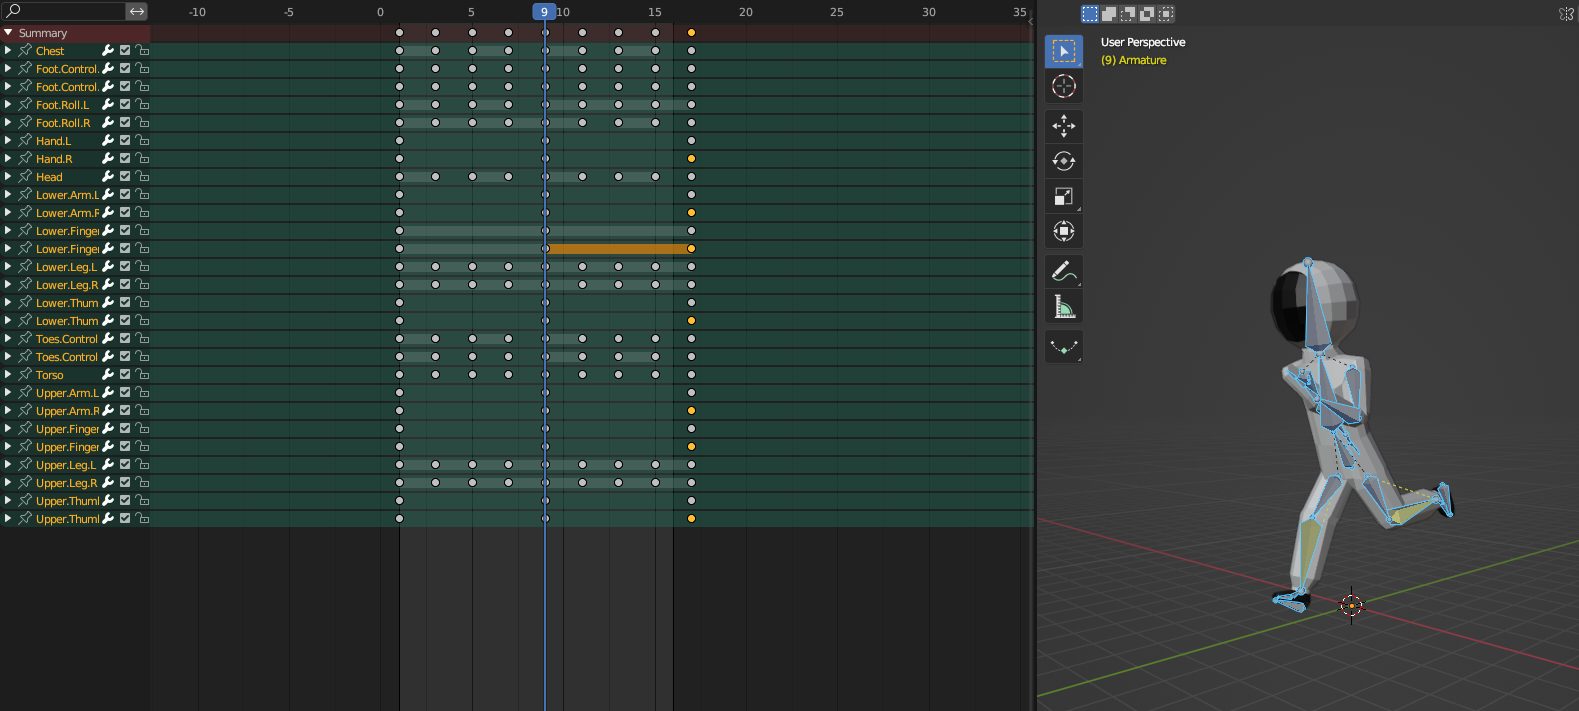
\includegraphics[width=0.8\textwidth]{chapters/theoretical_foundations/sections/models/resources/DopeSheet.png}
        \caption{Keyframes.}
        \label{fig:keyframes}
    \end{subfigure}

    \caption{Vertex weights and keyframes.}
\end{figure}

To define an animation a set of keyframes is used.
The process of creating the keyframes can be seen in \autoref{fig:keyframes}.
A keyframe is a set of transformations for each bone at a certain time.
Once the keyframes are defined the animation is interpolated between them to produce a smooth animation.
In the game, there are two animations: walking and running, both of which are looped to create a continuous animation when the player or an NPC moves.


The whole process of rendering an animation is as follows:
\begin{enumerate}
    \item The model along with the armature and keyframes are loaded into the game.
    \item A timer is started.
    \item The bone transformations for the current frame are calculated based on the keyframes and the timer.
    \item The bone transformations are passed into the shader.
    \item For each vertex the shader iterates over the bones that influence it and calculates the final position of the vertex based on the bone transformations and their weights.
    \item The animation is rendered.
\end{enumerate}